\documentclass[11pt, oneside]{article} 
\usepackage{geometry}
\geometry{letterpaper} 
\usepackage{graphicx}
	
\usepackage{amssymb}
\usepackage{amsmath}
\usepackage{parskip}
\usepackage{color}
\usepackage{hyperref}

\graphicspath{{/Users/telliott_admin/Dropbox/Tex/png/}}
% \begin{center} 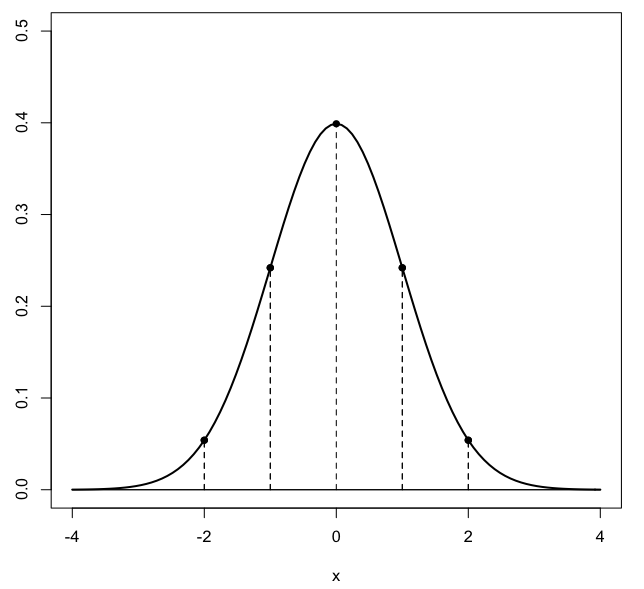
\includegraphics [scale=0.4] {gauss3.png} \end{center}

\title{Point and plane}
\date{}

\begin{document}
\maketitle
\Large

\subsection*{Construct a plane containing 3 points}

Consider three points 

$P = (1,0,0)$, $Q = (0,1,0)$, and $R = (0,0,1)$.  

Find two vectors in the plane by subtracting the second and third from the first.
\[ \mathbf{u} = (1,0,0) - (0,1,0) \]
\[ =  \ \langle 1,-1,0 \rangle \]
\[ \mathbf{v} = (1,0,0) - (0,0,1) \]
\[ = \ \langle 1,0,-1 \rangle \]

Obtain the normal vector by computing the cross product
\[ \mathbf{N} = \mathbf{u} \times \mathbf{v} 
\Rightarrow 
\begin{vmatrix}
\mathbf{\hat{i}} & \mathbf{\hat{j}}  & \mathbf{\hat{k}}  \\
1 & -1 & 0 \\
1 & 0 & -1 \\ 
\end{vmatrix} 
= 1 \mathbf{\hat{i}}  + 1 \mathbf{\hat{j}}  + 1 \mathbf{\hat{k}}  = \ \langle 1,1,1 \rangle  \]

One equation of the plane is then
\[ \mathbf{N} \cdot \mathbf{w} = 0 \] 
for any vector $\mathbf{w}$ in the plane.

Consider a fixed point in the plane ($x_0,y_0,z_0$).  Then any other point in the plane $(x,y,z)$ yields a vector from the fixed point which, dotted with $\mathbf{N}$, yields $0$
\[ \ \langle x-x_0,y-y_0,z-z_0 \rangle \  \cdot \  \langle 1,1,1 \rangle \ = 0 \]
\[ x - x_0 + y - y_0 + z - z_0 = 0 \]
\[ x + y + z = x_0 + y_0 + z_0 = d \]
Plugging in any one of the points yields
\[ x + y + z = d = 1 \]

\subsection*{find the closest point in the plane}

Consider any point in space, e.g. $P = (3,4,6)$.  

Find the point $Q$ on the plane which is closest to $P$, the point we arrive at by subtracting some fraction of $N$ from $P$.  

We have a point and a vector
\[ Q = P - t \mathbf{N} \]
\[ Q = (3,4,6) \ - \ t \langle 1,1,1 \rangle \ \]
Since $Q$ is in the plane, its components $x,y,z$ satisfy $x + y + z = 1$!  

So
\[ (3-t) + (4-t) + (6-t) = 1 \]
\[ 13 -3t = 1\]
\[ t = 4 \]
\[ Q = (-1,0,2) \]
Check that $Q$ is in the plane
\[ -1 + 0 + 2 = 1 \]
and $P-Q$ is parallel to $\mathbf{N}$
\[ P - Q = \ \langle 4,4,4 \rangle \]
that is definitely a multiple of $\mathbf{N}$.

\subsection*{point where a vector crosses the plane}

Where does the vector $\mathbf{w}$ that goes from the origin to point $P=(3,4,6)$ hit the plane?  Call that point $R$.  Again we have a point and a vector 
\[ R = (0,0,0) + t \mathbf{w} = (0,0,0) + t \ \langle 3,4,6 \rangle \]

And again, since $R$ is in the plane, its components $x,y,z$ satisfy $x + y + z = 1$.  So
\[ 3t + 4t + 6t = 1 \]
\[ t = \frac{1}{13} \]
\[ R = (\frac{3}{13}, \frac{4}{13}, \frac{6}{13}) \]

Notice that the vector $Q-R$ is in the plane, as it should be
\[ (Q-R) \cdot \mathbf{N} =  ((-1,0,2) - (\frac{3}{13}, \frac{4}{13}, \frac{6}{13})) \cdot \ \langle 1,1,1 \rangle \ \]
\[ =  \ \langle \frac{-16}{13}, \frac{-4}{13}, \frac{20}{13}> \  \cdot  \ \langle 1,1,1 \rangle  \ = 0 \]
And, adding the horizontal and vertical components together
\[ Q - R + P - Q = P - R = (3,4,6) - (\frac{3}{13}, \frac{4}{13}, \frac{6}{13}) \]
\[ = (\frac{36}{13}, \frac{48}{13}, \frac{72}{13}) \]
the result is parallel to $\mathbf{w}$.

\subsection*{Lines in space}

One way of specifying a line in 3D-space is as the intersection of two planes.  Another way is by giving a vector and a point in space.  Let's look at these in turn.
\noindent
Suppose we have the following two planes:
\[ x + y - z = 7 \]
\[2x - 3y + z = 3 \]

Since the $x,y,z$ terms are not related by a multiplicative constant, the planes are not parallel, so they will meet in a line, and the solutions consist of all the points on the line.  Let's find one solution, at $x=0$.  Then
\[ y - z = 7 \]
\[-3y + z = 3 \]
Adding
\[-2y = 10 \]
\[y = -5 \]
\[z = y - 7 = -12 \]
Our solution $P_0=(0,-5,-12)$.
Now find a second solution, at $z = -3$
\[ x + y = 4 \]
\[ 2x - 3y = 6 \]
Solving
\[ x = 4 - y \]
\[ 2(4-y) -3y = 6 \]
\[ 8 - 5y = 6 \]
\[ y = \frac{2}{5} \]
\[ x = \frac{18}{5} \]
The second point is $P_1 = (18/5, 2/5, -3)$.
Now we have two points on the line.  Its equation is 
\[ L = P_0 + t(P_1 - P_0) \]
\[ L = (0,-5,-12) + t(\frac{18}{5}, \frac{27}{5}, 9)\]
We can re-scale the vector that multiplies $t$ to have integer components (or length $1$, or whatever we wish).  Why not multiply by $5/9$?
\[ L = (0,-5,-12) + t(2, 3, 5)\]
There is another way to do this problem that might be a little easier.  Consider that the equation of the first plane gives its normal vector $n_1$ as
\[ n_1 =\ <1,1,-1> \]
Similarly the normal vector to the second plane is $n_2$
\[ n_2 =\ <2,-3,1> \]
Now, the vector that is parallel to the line of intersection is orthogonal to both $n_1$ and $n_2$  (Do you see why?)  So we compute the cross-product:
\[ n_1 \times n_2 = 
\begin{vmatrix} 
  i  &  j  &  k \\ 
  1  &  1 & -1 \\
  2  &  -3 & 1
\end{vmatrix}
\]
\[ = -2i -3j -5k \]
Multiplying by $-1$ gives what we obtained above.


\end{document}  